% !TeX root = ../../paper.tex
\subsection{Mini-Max-Suche}

Im Schachspiel ist jeder Spieler bestrebt, das für ihn bestmögliche Spielergebnis zu erzielen.
Zur Abbildung dieses Prinzips dient der \textit{Mini-Max}-Algorithmus [\cite{Paulsen2009}].
Um dies abbilden zu können wird ein Punktwert eingeführt, den ein Spieler zu maximieren versucht und der andere Spiele zu minimieren versucht.
Für das Schachspiel und die spätere Betrachtung dessen wird an dieser Stelle festgelegt, dass eine hohe Bewertungen für einen Vorteil der weißen Spielseite steht, wohingegen eine negative Bewertungen für einen Vorteil für die schwarze Spielseite steht.
Somit ist Weiß bestrebt, den Wert durch die Wahl einer Spieloption zu maximieren und Schwarz den Wert zu minimieren [\cite{Paulsen2009}].
Zur Berechnung dieses Punktwertes wird ein Spielbaum (engl. \textit{game tree}) benötigt, der alle möglichen Spielzüge beinhaltet.
Es werden alle Knoten eines Spielbaumes mit ihren zugehörigen Werten generiert [\cite{Shah2007}].
Die Knoten innerhalb des Baumes werden in drei verschiedene Kategorien unterteilt: Blattknoten, minierende und maximierende Knoten.
Jeder Blattknoten erhält seinen Nutzwert (engl. \textit{utility value}).
Den minimierenden Knoten wird jeweils der kleinste Wert ihrer Kindknoten zugewiesen, den maximierenden Knoten jeweils der größte Wert [\cite{Shah2007}].
Abbildung~\ref{fig:minimax_tic-tac-toe} zeigt einen Teil eines Spielbaums für das Spiel Tic-Tac-Toe, der die einzelnen Schritte der Berechnung durch den Mini-Max-Algorithmus beinhaltet.

\begin{figure}
    \centering
    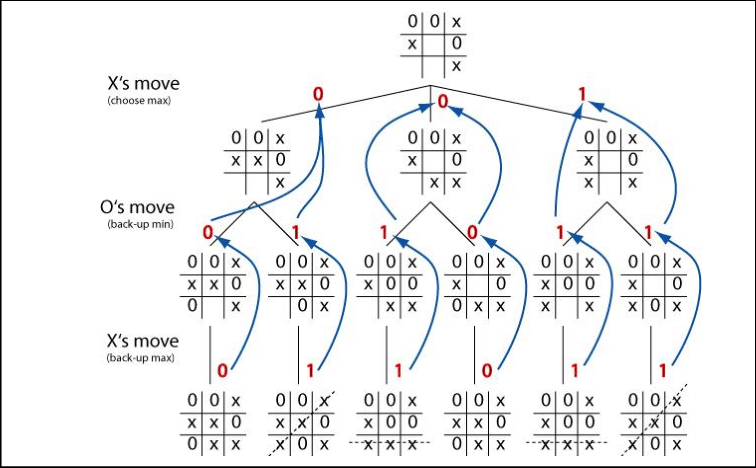
\includegraphics[width=0.89\textwidth]{images/theory/minimax_tic-tac-toe.png}
    \caption[Spielbaum eines Tic-Tac-Toe Spiels erstellt mittels des Mini-Max-Algorithmuses]{Spielbaum eines Tic-Tac-Toe Spiels erstellt mittels des Mini-Max-Algorithmuses [\cite{Elnaggar2014}]}
    \label{fig:minimax_tic-tac-toe}
\end{figure}

Die Ausgangssituation des Spiel ist an der Wurzel des Baumes abgebildet.
Im Falle des Spiels Tic-Tac-Toe wird festgelegt, dass Spieler X bestrebt ist, den Punktwert zu maximieren, wohingegen Spieler O bestrebt ist, diesen zu minimieren.
Spieler X ist als nächstes am Zug und besitzt drei Möglichkeiten, sein Kreuz auf dem Spielfeld zu platzieren.
Dem folgt der Spielzug des Spielers O, der seinerseits für jeden möglichen Spielzug von Spieler X je zwei Möglichkeiten besitzt, sein Symbol zu setzen.
Somit gibt es von der Ausgangslage her sechs mögliche Spielzüge, die Spieler O durchführen kann.
Zu guter Letzt hat Spieler X für jede seiner Ausgangslagen nur noch eine Möglichkeit, sein Kreuz zu setzen.
Jeder mögliche Endstand des Spiels erhält nun einen Punktwert.
Markiert der Endstand einen Sieg für Spieler X, so erhält dieser den Wert 1, bei einem Sieg für Spieler O den Wert -1 und bei einem Unendschieden den Wert 0.
Die Werte der Blattknoten werden anschließend nach oben propagiert.
Maximierende Knoten (Spieler X ist am Zug) übernehmen den jeweils höchsten Zahlenwert, minimierende Knoten (Spieler O ist am Zug) den niedrigsten Wert.
Am Ende dieses Prozesses ist von der Ausgangslage des Spiels erkennbar, dass Spieler X dem rechten Pfad des Baumes folgen muss, um garantiert einen Sieg zu erzielen, es für ihn aber auch bei einer Fehlentscheidung im nächsten Zug noch möglich ist, das Spiel zu gewinnen.
